\documentclass[
 reprint,
 superscriptaddress,
 amsmath,
 amssymb,
 aps,
]{revtex4-2}

\usepackage[colorlinks = true,
            linkcolor = blue,
            urlcolor  = blue,
            citecolor = blue,
            anchorcolor = blue]
            {hyperref}%
            
\usepackage{graphicx}% Include figure files
\graphicspath{ {./Assets/} }

\usepackage{dcolumn}%
\usepackage{bm}% bold math
\usepackage{titlesec}

\usepackage{listings}

\usepackage{xcolor}
\lstset { %
    language=C++,
    backgroundcolor=\color{black!5}, % set backgroundcolor
    basicstyle=\small,% basic font setting \small, \tiny, \footnsiz. \normalsize
}

\newcommand{\entryparam}[6]{
\subsubsection{#1}
\noindent
Type : #2\\
Unit : #3\\
Default-Value : #4\\
Pre-Condition : #5\\
Description : #6\\ }

\begin{document}

\title{Application programming interface of the Holovibes rendering engine}

\author{Julien Nicolle}
\author{Damien Didier}
\author{Sacha Bellier}
\author{David Chemaly}
\author{Adrien Langou}
\author{Philippe Bernet}
\author{Eliott Bouhana}
\author{Fabien Colmagro}
\author{Marius Dubosc}
\author{Guillaume Poisson}
\author{Michael Atlan}
\affiliation{
Centre National de la Recherche Scientifique (CNRS) UMR 7587, Institut Langevin. Paris Sciences et Lettres (PSL) University, Universit\'e Pierre et Marie Curie (UPMC), Universit\'e Paris 7. \'Ecole Sup\'erieure de Physique et de Chimie Industrielles ESPCI Paris - 1 rue Jussieu. 75005 Paris. France
}

\date{\today}

\begin{abstract}
This document describes the application programming interface (API) of the digital hologram rendering engine of the holovibes software. Guidelines for practical implementation of the API include a description of its logic, entry points, and usage. This software interface controls high bitrate digital hologram rendering and temporal demodulation from interference pattern streams from cameras or files by graphics processing units.
\end{abstract}

\maketitle

\tableofcontents

\section{\label{sec:intro} Introduction}

Holovibes is a digital hologram streaming software.\\
The increasing availability of ultra-fast cameras and graphic processing units (GPU) parallel computing power fuel the development of non-invasive digital holographic techniques that will predictably drive the democratization of compute-intensive imaging in real-time \cite{Leutenegger2011Real, samson2011video, Bencteux2015Holographic, Puyo2020Realtime}.
An application programming interface (API) is a way for two or more computer programs to communicate with each other. It is a type of software interface, offering a service to other pieces of software.[1] A document or standard that describes how to build or uses such a connection or interface is called an API specification. A computer system that meets this standard is said to implement or expose an API. The term API may refer either to the specification or to the implementation.\\
In contrast to a user interface, which connects a computer to a person, an application programming interface connects computers or pieces of software to each other. It is not intended to be used directly by a person (the end user) other than a computer programmer who is incorporating it into the software. An API is often made up of different parts which act as tools or services that are available to the programmer. A program or a programmer that uses one of these parts is said to call that portion of the API. The calls that make up the API are also known as subroutines, methods, requests, or endpoints. An API specification defines these calls, meaning that it explains how to use or implement them.\\
One purpose of APIs is to hide the internal details of how a system works, exposing only those parts a programmer will find useful and keeping them consistent even if the internal details later change. An API may be custom-built for a particular pair of systems, or it may be a shared standard allowing interoperability among many systems.\\
Our API work for the most part as a proxy to something called the 'Microcache' which is basically a container containing all states of all variables. Firstly, we will describe all entry points to the API. Then we will explain the execution flow of the API. It is recommended to read that part as it provides an in depth explanation of logs system and how to use the API.\\
The API is divided into different smaller 'cache'. These are inherent to how we handle different aggregate of variable. Technically you do not care about what is the cache that stores a particular variable, however, it could be useful to know because each cache as a specific theme (one for which windows are visible / another for compute settings ...) 

\begin{figure*}
    \centering
    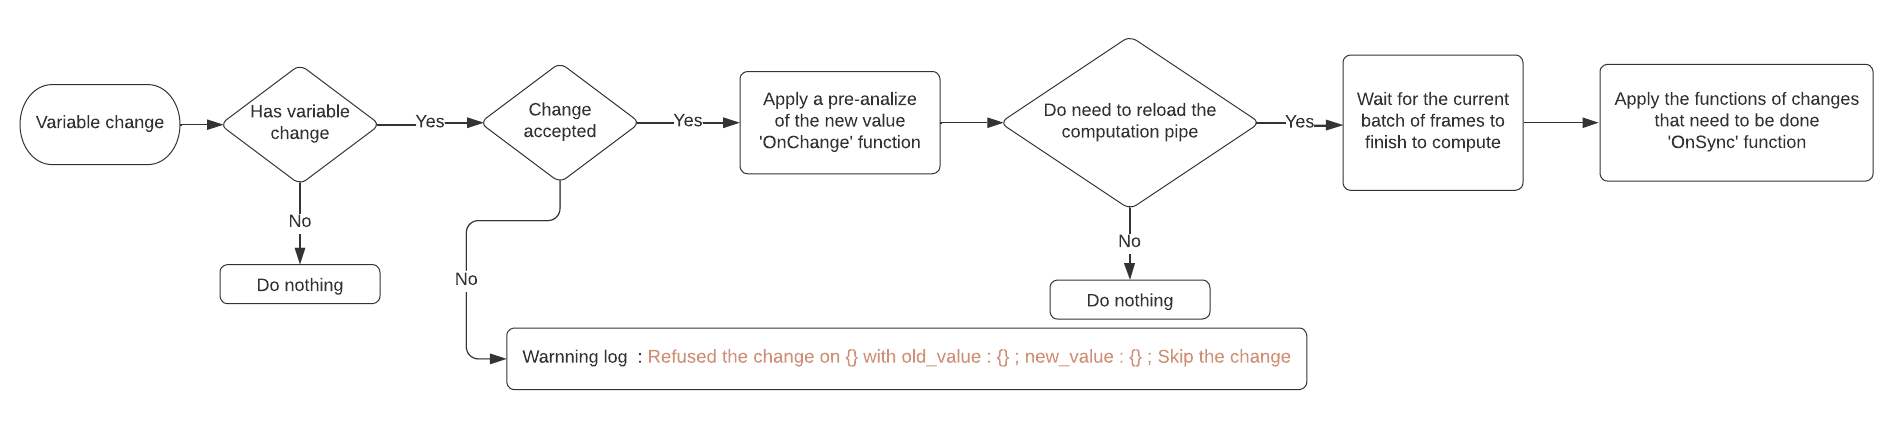
\includegraphics[width=\linewidth]{Holovibes, Microcache Pipeline.png}
    \caption{Caption}
    \label{fig_pipeline}
\end{figure*}

\section{API logic}

\subsection{Getters/Setters}
Before explaining all functions that are available, we will explain how our logic of getters / setters(Common method name in OOP[Object Oriented Programming] to get and set a specific field inside class, here our caches) works.\\
Our setters especially are complex because we want to execute all the 'Microcache' variable each time a variable changes and after all requests from the client are handled. For this, we have 3 types, two are really common : 

\begin{lstlisting}
T get_value<T>();
void set_value<T>(const T&);
\end{lstlisting}

The first one is for getting the value, you need 

\section{API Entry Points}
All the caches that we are speaking about are (remember that you don't have to know this to use the API, they are only useful to determine the theme of a variable)
\begin{itemize}
    \item AdvancedCache 
    \item ComputeCache
    \item ImportCache
    \item ExportCache
    %\item CompositeCache
    \item ViewCache
    %\item ZoneCache
\end{itemize}

Input variables / Computation settings
%\begin{AdvancedCache}

\subsection{AdvancedCache}

Advanced cache gathers all the (hidden) variables that can be set by advanced users, such as buffer sizes, and other parameters.
\begin{itemize}
    \item DisplayRate
    \item FileBufferSize
    \item InputBufferSize
    \item OutputBufferSize
    \item RecordBufferSize
    \item TimeTransformationCutsBufferSize
    \item Filter2DSmooth
    \item ContrastThreshold
    \item RenormConstant
    \item RawBitshift
    \item FrontEnd
\end{itemize}

\entryparam
    {DisplayRate}
    {Float}
    {Frames per second (Hz)}
    {24}
    {None}
    {This variable sets the refreshment rate of the real-time display(s) : main XY window, XZ and YZ cuts, lens view, raw frame view.}

\entryparam
    {FileBufferSize}
    {Integer}
    {Number of frames}
    {512}
    {None}
    {Specifies the size of the buffer used to read frame from input file.}

\subsubsection{InputBufferSize}
\noindent
Type : Integer\\
Unit : Number of frames\\
Default-Value : 512\\
Pre-Condition :  None\\
Description : Specifies the number of frames buffered in GPU VRAM queue, read from file or from camera stream, entering the image processing pipeline.\\

\subsubsection{OutputBufferSize}
\noindent
Type : Integer.\\
Unit : Number of frames.\\
Default-Value : 256\\
Pre-Condition : None\\
Description : Specifies the number of frames buffered in GPU VRAM queue for output.\\

\subsubsection{RecordBufferSize}
\noindent
Type : Integer\\
Unit : Number of images\\
Defaul-tValue : 1024\\
Pre-Condition : None\\
Description : Specifies the number of frames buffered in GPU VRAM queue exiting the image processing pipeline before being saved to disk.\\

\subsubsection{TimeTransformationCutsBufferSize}
\noindent
Type : Integer\\
Unit : Number of images\\
Default-Value : 512\\
Pre-Condition : None\\
Description : Specifies the number of frames buffered in GPU RAM queue, used for temporal demodulation.\\

\subsubsection{Filter2DSmooth}
\noindent
Type : Filter2DSmoothStruct \{ bool : enabled, int : low, int : high\}\\
Unit :  \\
Default-Value : \{ 0, 0 \}\\
Pre-Condition : None\\
Description : \\

\subsubsection{ContrastThreshold}
\noindent
Type : ContrastThresholdStruct  \{ float : lower, float : upper, uint : frame\_index\_offset\}\\
Unit : \\
Default-Value : \{ 0.5, 99.5, 2 \} \\
Pre-Condition : \\
Description : \\

\subsubsection{RenormConstant}
\noindent
Type : Integer\\
Unit : \\
Default-Value : 5\\
Pre-Condition : None \\
Description :\\

\subsubsection{RawBitshift}
\noindent
Type : Integer.\\
Unit : bits.\\
Default-Value :45\\
Pre-Condition : None\\
Shifts the bit content of two-byte encoding for display of less than 16-bit dynamic range raw data on the raw view.\\

\subsubsection{FrontEnd}
\noindent
Type : String\\
Unit : Name\\
Default-Value : ""\\
Pre-Condition : None\\
Description : Name of the linked front-end.\\

%\end{AdvancedCache}
%\begin{ComputeCache}

\subsection{ComputeCache}
\begin{itemize}
    \item ComputeMode
    \item ImageType
    \item BatchSize
    \item TimeStride
    \item Filter2D
    \item SpaceTransformation
    \item TimeTransformation
    \item TimeTransformationSize
    \item Lambda
    \item ZDistance
    \item Convolution
    \item PixelSize
    \item UnwrapHistorySize
    \item Unwrap2DRequested
    \item TimeTransformationCutsEnable
\end{itemize}

\subsubsection{ComputeMode}
\noindent
Type : Enum class ComputeModeEnum \{ Raw, Hologram \} \\
Unit : Input processes \\
Defaul-tValue : Raw \\
Pre-Condition : None\\
Description : Describe the behaviour of Holovibes. On raw no processing are done.\\

\subsubsection{ImageType}
\noindent
Type : Enum class ImageTypeEnum \{ Modulus, SquaredModulus, Argument, PhaseIncrease, Composite \}\\
Unit : \\
DefaultValue : Modulus\\
Pre-Condition : None\\
Description : Each ImageType provides access to some specific processing. Composite give access to RGB and HSV coloring. PhaseIncrease and Argument change the phase value (For all complex pixel c : atan(Im(c)/Re(c) and conjuguate of the phase between previous and current frame respectively)\\

\subsubsection{BatchSize}
\noindent
Type : Integer.\\
Unit : Number of frames.\\
DefaultValue : 1\\
Pre-Condition : None\\
Description : Sets the number of consecutive input frames onto which the spatial transformation is computed at once.\\

\subsubsection{TimeStride}
\noindent
Type : Integer.\\
Unit : Number of frames.\\
DefaultValue : 1\\
Pre-Condition : None\\
Description : Sets the number of input frame lag between two consecutive time transformations applied to the current data block.\\

\subsubsection{Filter2D}
\noindent
Type : Structure Filter2DStruct \{ bool : enabled, int : inner\_radius, int : outer\_radius\}\\
Unit : squared meters\\
DefaultValue : \{ false, 0, 1\}\\
Pre-Condition : None\\
Description : Apply a filter between main frames and the surface between squares of inner\_radius and outer\_radius size.\\

\subsubsection{SpaceTransformation}
\noindent
Type : Enum SpaceTransformationEnum \{ NONE, FFT1, FFT2 \}\\
Unit : calcul\\
DefaultValue : NONE\\
Pre-Condition : None\\
Description : FFT1 will apply one fft on batch\_size frames and apply a quadratic mask. FFT2 will apply one forward fft then a spectral mask and a reverse fft on batch\_size frames.\\

\subsubsection{TimeTransformation}
\noindent
Type : Enum TimeTransformationEnum \{ STFT, PCA, NONE, SSA\_FFT\}\\
Unit : calcul\\
DefaultValue : STFT\\
Pre-Condition : NONE\\
Description : The different TimeTransformation stands respectively for Shot-time Fourrier Transformation, Principal Component Analysis, no transformation, Self-adaptative Spectrum Analysis Short-time Fourrier Transformation. All are applied on time\_transformation\_size\\

\subsubsection{TimeTransformationSize}
\noindent
Type : Integer\\
Unit : Number of images\\
DefaultValue : 1\\
Pre-Condition : greater than 0\\
Description : Sets the number of input frames forming the data block onto which the time transformation is applied\\

\subsubsection{Lambda}
\noindent
Type : Float\\
Unit : nano-meters\\
DefaultValue : 852\\
Pre-Condition : None\\
Description : Optical radiation wavelength\\

\subsubsection{ZDistance}
\noindent
Type : Float\\
Unit : meters\\
DefaultValue : 1.5\\
Pre-Condition : None\\
Description : Hologram rendering/unfocus distance\\

\subsubsection{Convolution}
\noindent
Type : Struct ConvolutionStruct \{ bool : enabled, std::string : type, bool : divide, std::vector<float> : matrix \}\\
Unit : struct\\
DefaultValue : \{ false, "None", divide, []\}\\
Pre-Condition : None\\
Description : Bidimensional convolution of the current displayed image by a user-defined kernel.\\

\subsubsection{PixelSize}
\noindent
Type : Float\\
Unit : micro-meters\\
DefaultValue : 12\\
Pre-Condition : None\\
Description : Pixel pitch is the distance between center of adjacent pixels\\

\subsubsection{UnwrapHistorySize}
\noindent
Type : Integer\\
Unit : \\
DefaultValue : 1\\
Pre-Condition : None\\
Description : \\

\subsubsection{Unwrap2DRequested}
\noindent
Type :Boolean \\
Unit : \\
DefaultValue : false\\
Pre-Condition : None\\
Description : \\

\subsubsection{TimeTransformationCutsEnable}
\noindent
Type : Boolean\\
Unit : \\
DefaultValue : false\\
Pre-Condition : None\\
Description : \\

%\end{ComputeCache}
%\begin{ImportCache}

\subsection{ImportCache}
\begin{itemize}
    \item ImportType
    \item ImportFrameDescriptor
    \item ImportFilePath
    \item LoadFileInGpu
    \item StartFrame
    \item EndFrame
    \item FileNumberOfFrame
    \item LoopFile
    \item InputFps
    \item CurrentCameraKind
\end{itemize}

\subsubsection{ImportType}
\noindent
Type : Enum class ImportTypeEnum \{ None, File, Camera \}\\
Unit : struct
DefaultValue : None\\
Pre-Condition : None\\
Description : One the most important variable in Holovibes. It allow to run or not Holovibes.\\
\begin{itemize}
    \item None : Holovibes does not run and stop all workers if any were created. 
    \item File : Holovibes run using the data stream from the file 
    \item Camera : Holovibes run using the data stream from the configured camera 
\end{itemize}

\subsubsection{ImportFrameDescriptor}
\noindent
% Maybe Frame descritor could use uint16_t/uint32_t instead of short and int, we are in 2023... short are bad%
Type : class FrameDescriptor \{uint16\_t : width, uint16\_t : height, uint32\_t : depth, enum Endianness \{ LittleEndian, BigEndian \} byteEndian \} \\
Unit : struct
DefaultValue : { 0, 0, 0, LittleEndian }\\
Pre-Condition : None\\
Description : It is automatically set when you configure a camera or you load a file. Hence, it does not need to be edited manually.

\subsubsection{ImportFilePath}
\noindent
Type : String\\
Unit : Path\\
DefaultValue : ""\\
Pre-Condition : None\\
Description : Set the file to load. When this variable is changed, the new file at this path is loaded and all variables contained in the footer are loaded inside the Microcaches.

\subsubsection{LoadFileInGpu}
\noindent
Type : Boolean \\
Unit : None\\
DefaultValue : true \\
Pre-Condition : None\\
Description : When true, this variable indicates that the file to process has to be uploaded entirely in the GPU or split before beginning to send to the GPU. Set to false when the file is too large for GPU VRAM. If it's false then you can change the split size with the variable FileBufferSize in the AdvanceCache.

\subsubsection{StartFrame}
\noindent
Type : Integer \\
Unit : Frame index (Begin at 1). \\
DefaultValue : 1 \\
Pre-Condition : greater than 0 and lesser than FileNumberOfFrame\\
Description : Set the start index when reading through and accessing the input file\\

\subsubsection{EndFrame}
\noindent
Type : Integer\\
Unit : Frame index (Begin at 1)\\
DefaultValue : 1\\
Pre-Condition : greater than 0 and lesser than FileNumberOfFrame\\
Description : Set the end index reading through and accessing the input file\\

\subsubsection{FileNumberOfFrame}
\noindent
Type : Integer\\
Unit : Number of frames\\
DefaultValue : 1\\
Pre-Condition : greater than 0\\
Description : Total number of frames of the file. You shouldn not change this in normal case because it is automatically changed loading a file(by changing the ImportFilePath variable)\\

\subsubsection{LoopFile}
\noindent
Type : Boolean\\
Unit : None\\
DefaultValue : true\\
Pre-Condition : None\\
Description : Holovibes will either stop after reading the file until EndFrame or loop on it and start with the frame on index StartFrame\\

\subsubsection{InputFps}
\noindent
Type : Integer\\
Unit : Number of frames per seconds (fps)\\
DefaultValue : 60\\
Pre-Condition : 0\\
Description : Set the speed at which the file is read. Increasing it increases the computation power needed. Decreasing it will decrease the output fps\\

\subsubsection{CurrentCameraKind}
\noindent
Type : enum CameraKind \{ None or Adimec or IDS or Phantom or BitflowCyton or Hamamatsu or xiQ or xiB or OpenCV\}\\
Unit : enum \\
DefaultValue : None\\
Pre-Condition : None\\
Description : If different to None, Holovibes will edit ImportType variable to Camera and start the computation\\

%\end{ImportCache}
%\begin{ExportCache}

\subsection{ExportCache}
\begin{itemize}
    \item Record
    \item ExportScriptPath
    \item OutputFrameDescriptor
    \item ExportRecordDontLoseFrame
\end{itemize}

\subsubsection{Record}
\noindent
Type : Struct Record \{ std::string : file\_path, uint : nb\_to\_record, uint : nb\_to\_skip, bool : is\_running, enum RecordType \{ NONE or CHART or RAW or HOLOGRAM or CUTS\_XZ or CUTS\_YZ \} : record\_type \}\\
Unit : Struct\\
DefaultValue : \{ "", 0, 0, false, RAW\}\\
Pre-Condition : None\\
Description : Holds all information record related\\

\subsubsection{ExportScriptPath}
\noindent
Type : String\\
Unit : file path\\
DefaultValue : ""\\
Pre-Condition : None\\
Description : Script gpib used on record\\

\subsubsection{OutputFrameDescriptor}
\noindent
Type : Struct FrameDescriptor \{ ushort : width, ushort: height, uint : depth, Enum Endiannes \{ LittleEndian or BigEndian\} : byteEndian \}\\
Unit : struct\\
DefaultValue : \{ 0, 0, 0, LittleEndian\}\\
Pre-Condition : Describes record frames format\\

\subsubsection{ExportRecordDontLoseFrame}
\noindent
Type : Boolean\\
Unit : \\
DefaultValue : false\\
Pre-Condition : None\\
Description : Enforce Holovibes to wait frames on record\\
%\end{ExportCache}
%%\begin{CompositeCache}

\subsection{CompositeCache}
\begin{itemize}
    \item CompositeKind
    \item CompositeAutoWeights
    \item CompositeRGB
    \item CompositeHSV
\end{itemize}

\subsubsection{CompositeKind}
\noindent
Type : CompositeKindEnum \{ RGB, HSV \}\\
Unit : Define the kind of the representation of the colors \\
DefaultValue : RGB\\
Pre-Condition : \\

\subsubsection{CompositeAutoWeights}
\noindent
Type : Bool\\
Unit : \\
DefaultValue : false\\
Pre-Condition : \\

\subsubsection{CompositeRGB}
\noindent
Type : CompositeRGBStruct\{\}\\
Unit : \\
DefaultValue : CompositeRGBStruct\{\}\\
Pre-Condition : \\

\subsubsection{CompositeHSV}
\noindent
Type : CompositeHSVStruct{}\\
Unit : \\
DefaultValue : CompositeHSVStruct\{\}\\
Pre-Condition : \\

%\end{CompositeCache}
%\begin{ViewCache}

\subsection{ViewCache}
\begin{itemize}
    \item ViewAccuX
    \item ViewAccuY
    \item ViewAccuP
    \item ViewAccuQ
    \item ViewXY
    \item ViewXZ
    \item ViewYZ
    \item ViewFilter2D
    \item CurrentWindowKind
    \item LensViewEnabled
    \item ChartDisplayEnabled
    \item Filter2DViewEnabled
    \item FftShiftEnabled
    \item RawViewEnabled
    \item CutsViewEnabled
    \item RenormEnabled
    \item Reticle
\end{itemize}

\subsubsection{ViewAccuX}
\noindent
Type : struct ViewAccuXY \{ int : start, int : width \}\\
DefaultValue : \{ 0, 0 \}\\
Pre-Condition : None\\
Description : Used in 3D cuts to change the frequency viewed by Holovibes\\

\subsubsection{ViewAccuY}
\noindent
Type : struct ViewAccuXY \{ int : start, int : width \}\\
DefaultValue : \{ 0, 0 \}\\
Pre-Condition : None\\
Description : Used in 3D cuts to change the frequency viewed by Holovibes\\

\subsubsection{(ViewAccuP)ViewAccuZ}
\noindent
Type : struct ViewAccuPQ \{ int : start, int : width \}\\
DefaultValue : \{ 0, 0 \}\\
Pre-Condition : start + width need to be less than \verb|TimeTransformationSize|\\
Description : Used in 3D cuts to change the frequency viewed by Holovibes\\

\subsubsection{ViewAccuQ}
\noindent
Type : struct ViewAccuPQ \{ int : start, int : width \}\\
DefaultValue : \{ 0, 0 \}\\
Pre-Condition : None\\
Description : Used in 3D cuts to change the frequency viewed by Holovibes\\

\subsubsection{ViewXY}
\noindent
Type : struct ViewXYZ \{ bool : log\_enabled, bool : horizontal\_flip, float : rotation (0, 90, 180, 270), uint : output\_image\_accumulation \}\\
DefaultValue : \{ false, false, 0, 1 \}\\
Pre-Condition : None\\
Description : Information related to the first view\\

\subsubsection{ViewXZ}
\noindent
Type : struct ViewXYZ \{ bool : log\_enabled, bool : horizontal\_flip, float : rotation (0, 90, 180, 270), uint : output\_image\_accumulation \}\\
DefaultValue : \{ false, false, 0, 1 \}\\
Pre-Condition : None\\
Description : Information related to the view XZ, activated when \verb|CutsViewEnabled| is true\\

\subsubsection{ViewYZ}
\noindent
Type : struct ViewXYZ \{ bool : log\_enabled, bool : horizontal\_flip, float : rotation (0, 90, 180, 270), uint : output\_image\_accumulation \}\\
DefaultValue : \{ false, false, 0, 1 \}\\
Pre-Condition : None\\
Description : Information related to the view XZ, activated when \verb|CutsViewEnabled| is true\\

\subsubsection{ViewFilter2D}
\noindent
Type : struct ViewWindow \{ bool : log\_enabled, struct ViewContrast \{ bool : enabled, bool : auto\_refresh, bool : invert, float : min, float : max \}\}\\
DefaultValue : \{ false, \{ true, true, false, 1, 65535 \}\}\\
Pre-Condition : None\\
Description : Holds all information related to the filter2D view. \verb|log\_enabled| defined how contrast value are calculated, with logarithmic calculus or linear. \verb|ViewContrast| holds information related to contrast\\

\subsubsection{CurrentWindowKind}
\noindent
Type : enum WindowKind \{ ViewXY, ViewXZ, ViewYZ, ViewFilter2D \}\\
DefaultValue : ViewXY\\
Pre-Condition : None\\
Description : Which window is currently on focus\\

\subsubsection{LensViewEnabled}
\noindent
Type : bool\\
DefaultValue : false\\
Pre-Condition : None\\
Description : If true activates the lens view rendering and display\\

\subsubsection{ChartDisplayEnabled}
\noindent
Type : bool\\
DefaultValue : false\\
Pre-Condition : None\\
Description : If true activates the chart rendering and display\\

\subsubsection{Filter2DViewEnabled}
\noindent
Type : bool\\
DefaultValue : false\\
Pre-Condition : None\\
Description : If true activates the filter2d view rendering and display\\

\subsubsection{FftShiftEnabled}
\noindent
Type : bool\\
DefaultValue : false\\
Pre-Condition : None\\
Description : If true activates the fft shift on the main display(\verb|ViewWindowXY|)\\

\subsubsection{RawViewEnabled}
\noindent
Type : bool\\
Unit : None \\
DefaultValue : false\\
Pre-Condition : None\\
Description : If true activates the raw view display\\

\subsubsection{CutsViewEnabled}
\noindent
Type : bool\\
Unit : None \\
DefaultValue : false\\
Pre-Condition : None\\
Description : If true activates the ViewWindowXZ and ViewWindowYZ rendering and display\\

\subsubsection{RenormEnabled}
\noindent
Type : bool\\
Unit : None \\
DefaultValue : true\\
Pre-Condition : None\\
Description : If true renormalize the main window(ViewWindowXY)\\

\subsubsection{Reticle}
\noindent
Type : \\
Unit : \\
DefaultValue : \\
Pre-Condition : \\

%\end{ViewCache}
%%\begin{ZoneCache}

\subsection{ZoneCache}
\begin{itemize}
    \item SignalZone
    \item NoiseZone
    \item CompositeZone
    \item ZoomedZone
    \item ReticleZone
\end{itemize}

\subsubsection{SignalZone}
\noindent
Type : units::RectFd \\
Unit : Rectangle in the frame descriptor coordinates \\
DefaultValue : units::RectFd\{\} \\
Pre-Condition : \\

\subsubsection{NoiseZone}
\noindent
Type : units::RectFd \\
Unit : Rectangle in the frame descriptor coordinates \\
DefaultValue : units::RectFd\{\} \\
Pre-Condition : \\

\subsubsection{CompositeZone}
\noindent
Type : units::RectFd \\
Unit : Rectangle in the frame descriptor coordinates \\
DefaultValue : units::RectFd\{\} \\
Pre-Condition : \\

\subsubsection{ZoomedZone}
\noindent
Type : units::RectFd \\
Unit : Rectangle in the frame descriptor coordinates \\
DefaultValue : units::RectFd\{\} \\
Pre-Condition : \\

\subsubsection{ReticleZone}
\noindent
Type : units::RectFd \\
Unit : Rectangle in the frame descriptor coordinates \\
DefaultValue : units::RectFd\{\} \\
Pre-Condition : \\

%\end{ZoneCache}


\subsection{The Front-End API}

In order to get back images, we provide a front end API. The goal is that your are able to connect your front end that you created to Holovibes.
With this front end you will be able to connect callback for each modification.

We will provide you an example but there is some important thing to note about this API.

Firstly for each variable it provide you 2 callbacks, the first one is a before method and the second one is the after method. Between the two, there will be Holovibes logic. So why there are two callback is simple.

For example when the main output window begin, so you will need to wait that Holovibes create it, in that way you could create the after method in order to recover the newly created buffers to use it in your front end. You should not do that in the before because at this time the method of Holovibes was not call yet and thus the buffers may (and it's probably the case) not exist. 

And the before method exist for the other way, when this main windows is destroy, you should create the before method in order to unlink you (stop using the buffer stream) before this one get destroy in the Holovibes method. Same as before if you were unlink you in the after method method the buffers or the windows may (and it's probably the case) be destroy before you stop using it, and this will probably end up in a crash of your application.

\section{Microcache pipeline}



Firstly, most of the API functions are functions that used the Microcache pipeline. That why we are explaining it here.

\subsection{Microcache}
While Holovibes is computing your are able to change some of the computations setting, like the SpaceTransformation functions, the z distance, ...
The problem was that all of these variables are able to change only when Holovibes finish to do all current computation. Some variables doesn't do so much difficulties, like the z distance which can change almost anytime. But other like BatchSize need to free memory, allocate a new buffer, ...
And all of this cannot be done until we end using data stored in those buffers.
So we made Microcache which allow to specify all 'callbacks like functions' for each type of variable. With this system we are able to say that z distance can be change immediately, and vice versa for variables like batch size, which need to change buffers size, the Microcache is able to wait for that all the currents computed images to finish in order to apply the changes.

Don't be confused there is the Microcache's pipeline that we are describing here but there is also the compute pipe in Holovibes. The compute pipe it's just a list of all functions that will be applied for each batch of frames(of size BatchSize).

For each variables to see what has to be done, we run through a pipeline which is describe below.

\subsection{Pipeline}


This example show a preview of the Microcache's pipeline, each time a variable is changed or set, the hole pipeline is triggered.

Firstly if the variable doesn't change, because a pipeline run is costly, nothing will happen. If you want to force the all pipeline to be executed for a variable, a way to reload if you think that a setting is not correctly apply for example.

% This has to be check %
If you want to do it on import type for example(that what we use on the classic GUI to reload when start is repressed).


\begin{lstlisting}
    GSH::instance().import_cache()
    .force_trigger_param_W<ImportType>();
\end{lstlisting}

Then the 'change\_accepted' function is call, this function should not log a warning because in that case the new value is discard. You can check the different variables to see theirs conditions.

The 'OnChange' function will not be really use full for you. But it like preproccess the given value in order to re range it or to change other variables in reaction this change. For example when BatchSize change may be TimeStride need to change in order to work. It will in this function that the new value of TimeStride is set if the new value of BatchSize need it. 

By the way if you are linking a custom front end using the FrontEnd API, yours functions will be execute at the 'OnSync' function call. the before method will be before Holovibes OnSync method and yours front-end after method will be after the Holovibes one.


\section{New Data Types Created For Holovibes}
\subsection{Namespace Units}
Units is a namespace that contains RectFds.
\subsubsection{RectFds}
RectFds is a class that define a framedescriptor, it is a templated class by FdPixel, 
\subsubsection{Smooth}
RectFds is a class that define a framedescriptor
\subsubsection{Smooth2}


% ---
% ONECOLUMN STARTS
\onecolumngrid
\hfill
\noindent\rule[0.5ex]{\linewidth}{1pt}
% LINE AND SPACING

\section{Accessing and using the API}

\subsection{Connect a Front-end}

\subsection{Simplest use case}
To launch the API, there is almost only one variable that is important : InputType (in the InputCache)
This variable has 3 states
\begin{itemize}
    \item None : In that case, Holovibes is stopped and no worker is created.
    \item File : In that case Holovibes runs using the data stream from the file.
    \item Camera : In that case Holovibes runs using the data stream from the configured camera.
\end{itemize}

Remember that to change this value, you can use this
\begin{lstlisting}
    api::detail::set_value<ImportType>(ImportTypeEnum::File);
    or
    api::set_import_type(ImportTypeEnum::File);
\end{lstlisting}

\textbf{If you never change the value of \texttt{InputType}, Holovibes will never run.}

But only set it up is not sufficient, because you will need at least the stream to use.
If you are using a file, just set the \verb|ImportFilePath| variable
\begin{lstlisting}
    api::detail::set_value<ImportFilePath>("path/to/file.holo");
    or
    api::set_import_file_path("path/to/file.holo");
\end{lstlisting}

Of course you will need to do this before setting the import type variable.

% This part is not finish and need to be tested %

After following this section, you should have something like this
\begin{lstlisting}
    api::set_import_file_path("test.holo");
    api::set_import_type(ImportTypeEnum::File);
\end{lstlisting}

\subsection{Link a front-end}


% LINE AND SPACING
\noindent\rule[0.5ex]{\linewidth}{1pt}
\hfill
\twocolumngrid
% TWO COLUMN RESTARTS
% ---

\section{Conclusion}

This document describes the application programming interface (API) of the digital hologram rendering engine of the holovibes software. Guidelines for practical implementation of the API include a description of its logic, entry points, and usage. This software interface controls high bitrate digital hologram rendering and temporal demodulation from interference pattern streams from cameras or files by graphics processing units.\\

An application programming interface (API) is a way for two or more computer programs to communicate with each other. It is a type of software interface, offering a service to other pieces of software.[1] A document or standard that describes how to build or use such a connection or interface is called an API specification. A computer system that meets this standard is said to implement or expose an API. The term API may refer either to the specification or to the implementation.\\
In contrast to a user interface, which connects a computer to a person, an application programming interface connects computers or pieces of software to each other. It is not intended to be used directly by a person (the end user) other than a computer programmer who is incorporating it into the software. An API is often made up of different parts which act as tools or services that are available to the programmer. A program or a programmer that uses one of these parts is said to call that portion of the API. The calls that make up the API are also known as subroutines, methods, requests, or endpoints. An API specification defines these calls, meaning that it explains how to use or implement them.\\
One purpose of APIs is to hide the internal details of how a system works, exposing only those parts a programmer will find useful and keeping them consistent even if the internal details later change. An API may be custom-built for a particular pair of systems, or it may be a shared standard allowing interoperability among many systems.\\
Our API work for the most part as a proxy to something called the 'Microcache' which is a container of all states of all variables. We will first describe all entry points of the API. Then we will explain the 'Microcache' pipeline flow.\\
The API is divided into different smaller 'Microcache'. These are inherent to how we handle different aggregate of variables. Technically you do not need to know what cache stores a specific variable, however, it could be usefull to know because each cache as a specific theme (one for which windows are visible / another for compute settings ...) 

\section{Acknowledgements}

This work was supported by the French National research agency (ANR LIDARO and Laboratory of Excellence ANR-10-LABX-24), and the (\href{http://www.digitalholography.org}{digital holography foundation}).\\


\bibliographystyle{unsrt}
\bibliography{bibliography}



\end{document}
